\chapter{Conclusões e trabalhos subsequentes}\label{ch:conclusao}

Este capítulo apresenta na Seção \ref{sec:conclusao} as conclusões obtidas por
meio do desenvolvimento desta dissertação, à luz dos objetivos apresentados no
Capítulo \ref{ch:introducao}, mais especificamente nas seções
\ref{sec:obj_geral} e \ref{sec:obj_especificos}. Tais objetivos foram
desenvolvidos ao longo desta pesquisa de mestrado e seus resultados foram
apresentados nos capítulos \ref{ch:desenvolvimento} e \ref{ch:result}. Por fim,
são apontados pontos levantados como perspectiva para trabalhos futuros,
apresentados na Seção \ref{sec:futuro}.

\section{Conclusão}\label{sec:conclusao}

Este trabalho teve como principal objetivo o desenvolvimento do
\textit{Framework} PON C++ 4.0, orientado à programação genérica e utilização
recursos avançados de desenvolvimento em linguagem C++, introduzidos nos padrões
mais recentes da linguagem, como C++17 e C++20. Isto permitiu conceber uma
versão de \textit{framework} mais eficiente e fácil de se utilizar, no sentido
de ser menos \enquote{burocrático} e mais flexível, que os \textit{frameworks} em
linguagem C++ já existentes.

Em suma, a principal contribuição deste trabalho para o PON é a disponibilização
de um novo \textit{framework} para o desenvolvimento de aplicações em PON, o
\textit{Framework} PON C++ 4.0, que apresenta melhorias sobre as materializações
já existentes em linguagem de programação C++. O \textit{Framework} PON C++ 4.0
apresenta uma interface de programação que permite a representação do
conhecimento em mais alto nível, apresentando alto desemepenho em termos
de tempo de execução e permitindo a execução com paralelismo de forma estável,
de modo que ainda não era possível nas materializações anteriores.
% e mesmo os frameworks nas demais linguagens,
%nomeadamente C\#, Java, Akka e Erlang/Elixir.

Como parte dos objetivos, as principais melhorias apresentadas pelo
\textit{Framework} PON C++ 4.0, com relação aos \textit{frameworks} do PON em
C++ existentes, foram o suporte a execução \textit{multithread/multicore}
estável, adição de flexibilidade de tipos aos \textit{Attributes} e
flexibilidade algorítmica às \textit{Conditions}, além da redução da verbosidade
da utilização do \textit{framework}. O desenvolvimento do \textit{Framework} PON
C++ 4.0 também foi relatado sob a forma de um artigo no ICIST 2021
\cite{neves_icist_2021}.

O \textit{Framework} PON C++ 4.0 se inspira na estrutura e implementação do
\textit{Framework} PON C++ 2.0, no que tange as suas vantagens, permitindo
aproveitar a organização em padrões de projeto, como os padrões
\textit{Observer}, \textit{Iterator} e \textit{Singleton} que também estão
presentes nesta implementação, mas agora de forma mais pragmática no novo
\textit{framework}, além do padrão \textit{Builder} que foi adicionado no lugar
do padrão \textit{Factory}. Isto permitiu, dentre outros, redução de quantidade
de código em si no \textit{Framework} PON C++ 4.0 vis-à-vis o \textit{Framework}
PON C++ 2.0.

Neste âmbito, pode ser constatada, por meio da análise do código-fonte que
contém a implementação do \textit{Framework} PON C++ 4.0, quando comparado com a
versão do \textit{Framework} PON C++ 2.0, uma considerável redução do volume de
código utilizado para a implementação do \textit{framework} em si. Essa redução
no volume de código foi possível por meio da eliminação de estruturas de código
redundantes, devido à aplicação da programação genérica. Por exemplo, no caso da
implementação de \textit{Attributes} específicos para cada tipo, a implementação
com a utilização de \textit{templates} remove completamente a duplicidade de
código, o que também facilita a manutenção de código futuramente.

Além disso, a aplicação do método de desenvolvimento orientado a testes (TDD)
permite garantir que o \textit{Framework} PON C++ 4.0 possua o comportamento
correto nos casos de uso previstos para cada uma das entidades do PON. Os testes
disponíveis, além de garantir o funcionamento do \textit{framework} em seu
estado de desenvolvimento atual, servem como garantia que desenvolvimentos
futuros, como aqueles que serão propostos na Seção \ref{sec:futuro}, não
prejudiquem nenhuma das funcionalidades já existentes.  Ademais, o conjunto de
testes pode naturalmente ser expandido, conforme o desejo de grupos de
desenvolvedores.

Ainda, o trabalho desenvolveu aplicações de \textit{benchmark} para o
\textit{Framework} PON C++ 4.0. As aplicações desenvolvidas foram a aplicação de
sensores, aplicação de controle de semáforo, algoritmo \textit{Random Forest} e
algoritmo \textit{Bitonic Sort}. Tanto a aplicação de sensores como o controle
de semáforo são \textit{benchmarks} amplamente utilizados no grupo de pesquisas
do PON, enquanto os algoritmos \textit{Random Forest} e \textit{Bitonic Sort}
são ditos \textit{benchmarks} universalizados, por se tratar de algoritmos bem
estabelecidos e amplamente utilizados em uma variedade de linguagens de
programação e sistemas. Ainda, também houve o desenvolvimento de um jogo,
enquanto exemplo mais universal de aplicação. 

A aplicação de sensores permite principalmente comparar o desempenho do
\textit{Framework} PON C++ 4.0 com o \textit{Framework} PON C++ 2.0,
demonstrando ganhos significativos de desempenho sobre o mesmo, reduzindo tanto
o tempo de execução como consumo de memória das aplicações. Por sua vez, a
aplicação de controle de semáforo permitiu comparar a aplicação do paralelismo,
demonstrando a capacidade do \textit{Framework} PON C++ 4.0 de atingir alta
utilização dos núcleos disponíveis do processador, em níveis comparáveis aos
apresentados pelo \textit{Framework} PON C++ Elixir/Erlang. 

Com os \textit{benchmarks} universalizados desenvolvidos, por meio dos
algoritmos \textit{Random Forest} e \textit{Bitonic Sort}, foi possível
demonstrar a viabilidade da utilização do PON, mais especificamente com o
\textit{Framework} PON C++ 4.0, para o desenvolvimento de aplicações bem
estabelecidas, mesmo que o desempenho ainda seja inferior ao das implementações
com a linguagem C no PP, o que absolutamente natural em função do caráter
arquétipal de \textit{framework} e deve ser resolvido quando a Tecnologia
LingPON estiver mais próxima de estado da técnica do que estado da arte. Em todo
caso, ainda nestes \textit{benchmarks} também foi demonstrada a capacidade de
execução \textit{multithread} do \textit{Framework} PON C++ 4.0. 

Neste âmbito, espera-se que estas implementações motivem trabalhos subsequentes
do PON, incluindo com a emergente Tecnologia LingPON, a adotarem o uso destes
\textit{benchmarks} universalizados, visto que este trabalho demonstra sua
viabilidade para tais implementações. Na verdade, já se observa no grupo de
pesquisa a tendência a uso de benchmarks universalizados, por influência deste
trabalho, bem como dos trabalhos de Pordeus
\cite{quali_pordeus_2020,pordeus_2020,pordeus_2021}, com \textit{benchmarks} em PON em
\textit{hardware} que influenciaram este presente trabalho neste âmbito.

Isto dito, além das aplicações de \textit{benchmark} universalizados e também do
grupo desenvolvidas com o propósito de avaliar o \textit{Framework} PON C++ 4.0
do ponto de vista de desempenho, também houve o desenvolvimento de um jogo com
\textit{NOPUnreal}. Este jogo já havia sido implementado pelo próprio autor
deste trabalho dissertação, conforme \citeonline{neves_2020}, sendo então
reimplementado com o \textit{Framework} PON C++ 4.0. Esta aplicação serve
inclusive como demonstração do uso do \textit{Framework} PON C++ 4.0 para o
desenvolvimento de uma aplicação complexa, com um grande número de
\textit{Rules} em sua composição.

O desenvolvimento dessa aplicação de jogo com \textit{NOPUnreal} permitiu também
demonstrar em algo a redução da verbosidade do \textit{Framework} PON C++ 4.0
quando comparado com o \textit{Framework} PON C++ 2.0, que pode ser constatada
pela redução de linhas de código desta nova implementação do jogo. A
implementação com o \textit{Framework} PON C++ 4.0 resultou em um total de 1514
linhas de código, o que significa 258 linhas de código a menos que a mesma
implementação com o \textit{Framework} PON C++ 2.0. Ainda que subjetivo, este
resultado aliado aos demais, permitem estabelecer a redução de verbosidade enfim
com o aqui proposto \textit{Framework} PON C++ 4.0.

No que diz respeito aos avanços promovidos pelo \textit{Framework} PON C++ 4.0
no sentido de facilitar a programação, do ponto de vista de desacoplamento, a
implementação com \textit{smart pointers} contribui ao facilitar o gerenciamento
de memória. Isto porque possibilita a criação de elementos de forma dinâmica em
qualquer lugar do código e permite também o compartilhamento de forma simples em
diversos pontos do código, até mesmo em \textit{threads} diferentes. Assim, este
recurso foi fundamental como construto para o \textit{Framework} PON C++ 4.0 como um
todo.

Em geral, o uso de \textit{smart pointers} tem como principal benefício o
gerenciamento de memória de forma transparente ao desenvolvedor e, com isto,
existe a garantia de que não haverá vazamento de memória, evitando muitos
problemas que podem ocorrer em tempo de execução, como ocorre em versões
anteriores, particularmente do \textit{Framework} PON C++ 2.0, conforme
observado na Seção \ref{sec:perf_test}. Esses benefícios também se aplicam em
ambientes \textit{multithread}, pois os \textit{shared pointers} utilizam
contadores atômicos para o controle do número de referências, minimizando os
problemas decorrentes ao acesso de recursos compartilhados entre as
\textit{threads}, como aqueles observados no Framework PON C++ 3.0.

A complexidade adicionada ao \textit{framework} decorrente da aplicação de
conceitos de programação genérica e uso dos recursos avançados da linguagem C++
é transparente ao desenvolvedor do PON, que fará a utilização do
\textit{Framework} PON C++ 4.0, devido à existência de abstrações, como as
interfaces de construção de entidades por meio de \textit{builders}. Desta
forma, o desenvolvedor do PON que deseja utilizar o \textit{Framework} PON C++
4.0 necessita conhecer apenas as interfaces genérica e de uso simples oferecidas
pelo \textit{framework}. A facilidade de programação, que é um critério
subjetivo, foi corroborada por meio da opinião de desenvolvedores do grupo de
pesquisa do PON, conforme apresentado na Seção \ref{sec:opiniao}, enquanto pode
ser observada \textit{in loco} nos exemplos que foram apresentados ao longo da
dissertação.

Com a facilitação da programação em PON apresentada pelo \textit{Framework} PON
C++ 4.0, no sentido de desenvolvimento desburocratizado e em alto nível,
espera-se obter maior engajamento dos desenvolvedores no uso do PON para o
desenvolvimento de suas aplicações, principalmente no contexto das disciplinas
de PON na UTFPR, de forma a ampliar o número de aplicações desenvolvidas em PON,
ajudando a corroborar os aspectos teóricos do PON e demonstrando sua pertinência
em aplicações cada vez mais práticas e realísticas. Neste âmbito, a redução na
verbosidade da utilização do \textit{framework} contribui principalmente na
redução do número de linhas de código utilizadas no desenvolvimento destas
aplicações com o \textit{Framework} PON C++ 4.0 e também tem como benefício
simplificar as aplicações e potencialmente reduzir o tempo de desenvolvimento
das mesmas.

Ademais, é importante observar como o \textit{Framework} PON C++ 4.0 se
apresenta como uma evolução sobre as materializações existentes em
\textit{frameworks} com C++, materializando a propriedade de paralelização que
não era atingida pelo \textit{Framework} PON C++ 2.0 e, finalmente, não
efetivamente nem mesmo em \textit{Framework} PON C++ 3.0, enquanto também
apresenta as mesmas funcionalidades e conceitos de programação disponíveis no
\textit{Framework} PON C++ 2.0/3.0, com exceção do conceito de impertinência e
\textit{Keeper}, devido aos motivos apresentados na Seção \ref{sec:reflex}.

Em suma, dadas todas as evoluções apresentadas no estado da técnica
desenvolvidas neste trabalho e no estado da arte com comparações via
\textit{benchmarks} fidedignos, pode-se dizer que as demandas de desenvolvimento
de \textit{software} apresentadas como motivação para o desenvolvimento deste
trabalho, já apresentadas na Seção \ref{sec:motiv}, de desenvolvimento em alto
nível, com alto desempenho e paralelismo são atendidas pelo \textit{Framework}
PON C++ 4.0 enquanto arquétipo de paradigma de programação/desenvolvimento
emergente. Ainda, no que diz respeito ao atendimento dessas demandas, o
\textit{Framework} PON C++ 4.0 se mostra superior aos demais \textit{frameworks}
do PON disponíveis. Por fim, pode ser dito que a maior contribuição deste
trabalho do ponto de vista técnico é ainda a disponibilização, sob a forma do
\textit{Framework} PON C++ 4.0, de uma ferramenta com caráter profissional que
facilita o desenvolvimento de aplicações sob a luz do Paradigma Orientado a
Notificações e que foi devidamente demonstrando no âmbito de uma pesquisa de
mestrado.

\section{Trabalhos subsequentes}\label{sec:futuro}

O presente trabalho apresenta o \textit{Framework} PON C++ 4.0 como
uma versão mais madura e estável de \textit{framework} a ser utilizada tanto
como base para o desenvolvimento de aplicações em PON como para a evolução da
tecnologia de \textit{frameworks} em si. Espera-se que o
\textit{Framework} PON C++ 4.0 tenha ampla utilização no
desenvolvimento dos trabalhos futuros do grupo de pesquisa do PON.

Durante o desenvolvimento deste trabalho foram vislumbradas diversas
possibilidades para o desenvolvimento de outros trabalhos pertinentes, mas que
fogem do escopo desta dissertação, de forma que são deixados como propostas para
trabalhos futuros. Estas propostas são detalhadas nas seções seguintes.

\subsection{Desenvolvimento de aplicações com o \textit{Framework} PON C++ 4.0}

Ainda neste trabalho foram demonstrados diversos casos de uso com o
\textit{Framework} PON C++ 4.0, por meio da aplicação de sensores, aplicação de
controle de semáforos, algoritmo \textit{Bitonic Sort}, algoritmo \textit{Random
Forest} e do jogo \textit{NOPUnreal}. Essas aplicações, apesar de demonstrarem o
potencial de utilização do \textit{Framework} PON C++ 4.0 em diversos contextos,
inclusive e particularmente do ponto de vista de pesquisa, ainda tem escopo
limitado do ponto de vista industrial, sendo consideradas aplicações simples do
ponto de vista de desenvolvimento de \textit{software}.

Como uma das motivações para o desenvolvimento do \textit{Framework} PON C++ 4.0
era justamente possibilitar o desenvolvimento de aplicações mais complexas,
devido à facilitação do uso do \textit{framework} em si, se torna pertinente o
desenvolvimento de tais aplicações. Isto de forma tal a consolidar não somente o
\textit{Framework} PON C++ 4.0 como também a aplicação do PON ao desenvolvimento
de \textit{software} no contexto industrial ou similar, além do contexto de
\textit{benchmarks} de pesquisa, \textit{benchmarks} estes que justamente
serviram de viabilizadores para ensejar tais aplicações com caracteres
industriais. Nesse sentido, já está em andamento trabalho de Abu Ahmed Babu que
visa aplicar o Framework PON C++ 4.0 em sistemas sencientes ou afins,
possivelmente uma \textit{smart-house}, com olhar sobre computação verde.

Neste sentido destaca-se a possibilidade do desenvolvimento de uma nova versão
do futebol de robôs, anteriormente implementado por \citeonline{msc_santos_2017}
e também por \citeonline{lima_2020} com o \textit{Framework} PON C++ 2.0, que
agora pode ser implementado com o \textit{Framework} PON C++ 4.0 como
viabilizador para aplicações industriais devido a suas complexidades e escalas.
Ainda neste escopo, também poderia ser desenvolvida a NeuroPON conforme
\citeonline{doc_Schutz_2019} e PONFuzzy conforme \cite{msc_melo_2016} e suas
aplicações em Framework PON C++ 4.0.

Por fim, \citeonline{skora_2021} também propõe a utilização do PON, por meio do
\textit{Framework} PON C++ 4.0 para o desenvolvimento de um analisador
léxico-sintático. Ainda, esta aplicação apresenta um caráter preliminar,
necessitando ser evoluída.

\subsection{Compilador LingPON com alvo \textit{Framework} PON C++ 4.0}

Ainda durante o próprio desenvolvimento desta dissertação, foi desenvolvido um
novo alvo de compilação da LingPON para o \textit{Framework} PON C++ 4.0,
implementado por \citeonline{skora_2020}. A estrutura similar à do
\textit{Framework} PON C++ 2.0, porém ainda mais genérica e fácil de utilizar,
facilita o desenvolvimento de um novo alvo de compilação para a LingPON.

Ademais, existem esforços direcionados no sentido de melhorar a LingPON,
permitindo a criação dinâmica de entidades \cite{oshiro_2021}. Os
\textit{frameworks} do PON atuais ainda não dão suporte a esta criação dinâmicas
de entidades, que seria viabilizada com a compilação para o \textit{Framework}
PON C++ 4.0, assim como a possível adoção do conceito de \textit{Condition} com
flexibilidade algorítmica na LingPON.

\subsection{\textit{Framework} PON C++ 4.0 Distribuído}\label{sec:pon_dist}

Diversos estudos afirmam e mesmo demonstram que o PON pode ser facilmente
utilizado em sistemas distribuídos
\cite{msc_Banaszewski_2009,talau_2016,barreto_2018,oliveira_2018,msc_oliveira_2019,msc_negrini_2019,martini_2019},
de forma que um desenvolvimento pertinente seria a implementação da propriedade
de distribuição no \textit{Framework} PON C++ 4.0. Conforme mostrado na Figura
\ref{fig:pon_dist}, a propriedade de distribuição no PON permite a execução das
entidades do PON, como \textit{Premises} e \textit{Attributes}, de forma
transparente ao sistema em ambientes distintos.

\begin{figure}[!htb]
\centering
\caption{Comunicação distribuída com o PON}
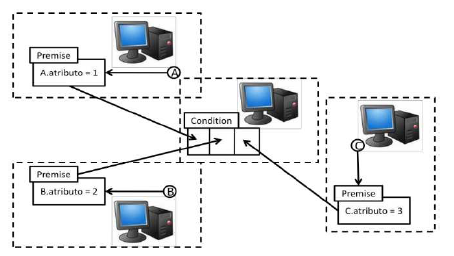
\includegraphics[width=0.8\textwidth]{../figures/pon_dist.PNG}
\smallskip
\caption*{Fonte: \citeonline{msc_Banaszewski_2009}}
\label{fig:pon_dist}
\end{figure}

Como apresentado na Seção \ref{sec:reflex}, mais especificamente na Tabela
\ref{tab:elementares_2}, o \textit{Framework} PON C++ 4.0 materializa as
propriedades de programação em alto nível, paralelismo e desempenho do PON,
porém esta implementação ainda não materializa a propriedade de distribuição.
Desta forma, já é previsto o desenvolvimento de pesquisa considerando a
implementação de mecanismos que possibilitem atender a propriedade de
distribuição com o \textit{Framework} PON C++ 4.0. Já existe inclusive trabalho
de mestrado em andamento desenvolvimento por Pelegrin Figueiredo nesse
tópico.

A implementação do mecanismo de distribuição no \textit{Framework} PON C++ 4.0
pode ser feita aproveitando os conceitos apresentados, por exemplo, pelo PON
\textit{internet protocol} (PONIP) \cite{talau_2016}. O PONIP apresenta um
esquema independente de materialização para a comunicação via protocolo IP entre
entidades do PON. Apesar de limitado, possibilitando a distribuição apenas de
\textit{Premises} e \textit{Attributes} de tipos básicos, ele já oferece uma
base para o desenvolvimento de aplicações distribuídas com o PON.

O PONIP poderia ser utilizado diretamente com o \textit{Framework} PON C++ 4.0,
porém, de forma a manter o nível de abstração e facilidade de programação
propostos pelo \textit{Framework} PON C++ 4.0, uma implementação de distribuição
nativa ao \textit{Framework} PON C++ 4.0 seria mais interessante, ainda que seja
implementada aproveitando os conceitos do PONIP.

\subsection{NeuroPON}\label{sec:neuropon_futuro}

O NeuroPON, conforme apresentado na Seção \ref{sec:fw3}, foi implementado
utilizando o \textit{Framework} PON C++ 3.0, buscando aproveitar os benefícios
que seriam possibilitados pela aplicação do paralelismo possibilitado com tal
\textit{framework}. Entretanto, foi visto que a implementação de paralelismo no
\textit{Framework} PON C++ 3.0 não apresenta resultados esperados no que diz
respeito ao desempenho das aplicações.

Nesse sentido, seria interessante a implementação do NeuroPON com o
\textit{Framework} PON C++ 4.0, visto que, conforme os resultados apresentados
no Capítulo \ref{ch:result}, o \textit{framework} possibilitou observar ganhos
de desempenho na aplicação \textit{Bitonic Sort}, sendo possível vislumbrar
eventuais ganhos de desempenho com a paralelização na aplicação do NeuroPON.

\subsection{Técnicas de depuração em PON}\label{sec:debug_futuro}

Uma das principais dificuldades apresentadas no desenvolvimento de
\textit{software} em PON é a dificuldade de depuração do código. Essa
dificuldade advem do fluxo de execução não sequencial das aplicações em PON, que
dificulta o uso de ferramentas de depuração usualmente disponíveis para as
principais linguagens de programação.

Nesse sentido, o \textit{Framework} PON C++ 4.0, seguindo o que já havia sido
proposto com o \textit{Framework} PON C++ 2.0, apresenta um mecanismo de
registro de \textit{logs} que permitem ao desenvolvedor analisar a execução do
\textit{software}. Entretanto, o uso de tais ferramentas ainda tem efetividade
limitada, de modo que o PON carece de ferramentas mais avançadas para a
depuração de \textit{software}.

Uma possibilidade vislumbrada para auxiliar depuração em PON é a criação de uma
ferramenta que permita observar de forma gráfica esse fluxo de execução do
\textit{software} que é registrado por meio de \textit{logs}. Tal ferramenta
poderia utilizar como base os registros já existentes, interpretando e
fornecendo ao desenvolvedor uma interface mais fácil de se analisar.
